\documentclass{article}
\usepackage{tikz}
\usepackage{amssymb,amsmath,amsthm}
\usepackage{fullpage}
\usepackage{algorithm}
\usepackage{algorithmic}
\newcommand{\FCC}{C}
\DeclareMathOperator*{\argmin}{arg\,min}
\DeclareMathOperator*{\argmax}{arg\,max}
\DeclareMathOperator*{\maximize}{maximize}
\DeclareMathOperator*{\minimize}{minimize}
\newcommand{\ZZ}{\mathbb Z}
\newcommand{\NN}{\mathbb N}
\newcommand{\RR}{\mathbb R}
\newtheorem{theorem}{Theorem}
\newtheorem{definition}{Definition}

\title{Supplementary material for ``A log-linear time segmentation algorithm for peak detection in genomic data''}

\begin{document}

\maketitle

\section*{Supplementary Figure 1}
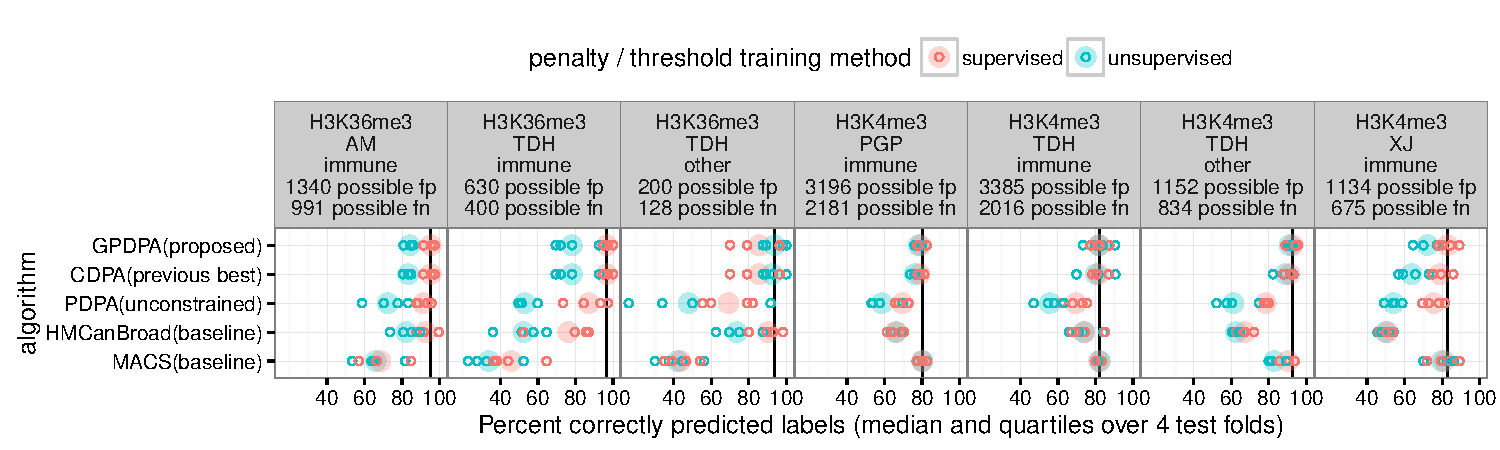
\includegraphics[width=\textwidth]{figure-test-error-dots-supp}
Four-fold cross-validation was used in each of seven data sets to
estimate peak detection accuracy, in terms of percent incorrect
labels. For unsupervised learning, default significance thresholds
were used for HMCanBroad (finalThreshold=10) and MACS (qvalue=0.05);
elbow/hinge heuristic for oracle penalty was used for PDPA/CDPA/GPDPA,
as implemented in Segmentor3IsBack R package (Cleynen and Lebarbier,
2014). For supervised learning, thresholds and penalty constants were
as described in the main text. Counts of possible fp and fn are for
all labels in that data set (possible fp are any labels which could
possibly have a false positive, etc); possible fp is always greater
than possible fn, indicating that all data sets are unbalanced in the
same direction (more negative labels than positive labels).

\section{Proof of optimality of dynamic programming algorithm}

\subsection{Reminder of relevant definitions}

Let $y_1,\dots,y_n$ be a sequence of $n$ data points to segment. The
optimization space for the reduced isotonic regression model with $K$
segments is
\begin{definition}
\label{def:Ibar}
  Let $(\mathbf u, \mathbf t)\in{\mathcal I}_n^K$ be the set of
  all non-decreasing segment means $u_1\leq\cdots\leq u_K$ and
  increasing changepoint indices $0=t_0<t_1<\cdots<t_{K-1}<t_K=n$.
\end{definition}
Each segment
mean $u_k$ is assigned to data points
$\tau\in(t_{k-1},t_k]\subset\{1,\dots,n\}$, resulting in the following
cost for each segment $k\in\{1, \dots, K\}$,
\begin{equation}
  \label{eq:h}
  h_{t_{k-1}, t_k}(u_k) = \sum_{\tau=t_{k-1}+1}^{t_k} \ell(y_\tau, u_k),
\end{equation}
where $\ell:\RR\times\RR\rightarrow\RR$ is a convex loss function.
The optimal cost functions are defined as
\begin{definition}
\label{def:fcc}
  We define $\FCC_{K,n}(\mu)$ the optimal cost of the segmentation
  with $K$ segments, up to data point $n$, with last segment mean
  $\mu$. In other words:
%% we take the minimum with the constraint that the last mean (u_k) is mu
\begin{equation}
\FCC_{K,n}(\mu) = \min_{(\mathbf u, \mathbf t)\in{\mathcal I}_n^K \ | \ u_K = \mu} \
  \left\{ \sum_{k=1}^K
  h_{t_{k-1}, t_k}(u_k) \right\}
\end{equation}
\end{definition}
For
any function $f:\RR\rightarrow\RR$, we define the min-less operator as
\begin{equation}
  \label{eq:min-less-def}
  f^\leq(\mu)=\min_{x\leq \mu} f(x).
\end{equation}

\subsection{Proof of update rules}

\begin{theorem}
  The optimal cost functions can be recursively computed using the
  following dynamic programming update rules.
\begin{enumerate}
\item For $K=1$ we have
$\FCC_{1,1}(u)=\ell(y_1,u)$, and for the other data
  points $t>1$ :
\begin{equation}
\FCC_{1,t}(u)=\FCC_{1,t-1}(u)+\ell(y_t,u)
\end{equation}

\item For $K>1$ and $t=K$
\begin{equation}
  \FCC_{K,t}(u)=\ell(y_K, u)+\FCC_{K-1,K-1}^\leq(u)
\end{equation}
\item In all other cases we have
  \begin{equation}
  \FCC_{K,t}(u)=\ell(y_t,u)+
  \min\{
  \FCC_{K-1,t-1}^\leq(u),\,
  \FCC_{K,t-1}(u)
  \}.
  \end{equation}
\end{enumerate}
\end{theorem}

%% we now prove the lemma
%% Case 1 and 2 are true almost by definition 
%% (there is only one possible segmentation in 1) and 
%% (there is only possible segmentation in K of K points)
\begin{proof}
Case 1 and 2 follow from the definition of $\FCC_{K,t}(u)$.

We now focus on case 3.
First notice that by definition of $\FCC_{K,t+1}(u)$ (i.e. the optimal segmentation) we must have
$\FCC_{K,t+1}(u) \leq \FCC_{K,t}(u) + \ell(y_t,u)$ and also
$\FCC_{K,t+1}(u) \leq \FCC_{K-1,t}(u) + \ell(y_t,u)$. Thus we have
$\FCC_{K,t+1}(u) \leq \min \{ \FCC_{K,t}(u) , \FCC_{K-1,t}(u) \} + \ell(y_{t+1},u)$.

Now let us assume,
$$\FCC_{K,t+1}(u) < \min \{ \FCC_{K,t}(u) , \FCC_{K-1,t}(u) \} + \ell(y_{t+1},u).$$
We will show that this lead to a contradiction.

We consider the optimal segmentation
$(\mathbf u, \mathbf t)\in{\mathcal I}_{t+1}^K$ which achieves the
optimum of $\FCC_{K,t+1}(u)$. We consider two possible cases:
\begin{description}
\item[Scenario 1: $t_K < t$.]  Define $\mathbf t'$ such that for all
  $i < K$, we have $t'_i = t_i$ and $t'_K = t$.  We have
  $(\mathbf u, \mathbf t')\in{\mathcal I}_{t}^K$.  We can thus
  decompose $\FCC_{K,t+1}(u)$ as

$$\FCC_{K,t+1}(u) = \sum_{k=1}^K
  h_{t'_{k-1}, t'_k}(u_k) + \ell(y_{t+1},u).$$ 

By assumption we would recover $\sum_{k=1}^K h_{t'_{k-1}, t'_k}(u_k) < \FCC_{K,t}(u)$ which is a contradiction
by definition of $\FCC_{K,t}(u)$. 

\item[Scenario 2: $t_K=t$.]  Define $\mathbf t'$ such that for all
  $i < K-1$, we have $t'_i = t_i$ and $t'_{K-1} = t$. Also define
  $\mathbf u'$ such that for all $k \leq K-1$, we have $u'_k = u_k$.
  Thus $(\mathbf u', \mathbf t')\in{\mathcal I}_{t}^{K-1}$, and can
  then decompose $\FCC_{K,t+1}(u)$ as

$$\FCC_{K,t+1}(u) = \sum_{k=1}^K
  h_{t'_{k-1}, t'_k}(u'_k) + \ell(y_{t+1},u).$$ 

By assumption we would recover $\sum_{k=1}^{K-1} h_{t'_{k-1}, t'_k}(u'_k) < \FCC_{K-1,t}(u)$ which is a contradiction
by definition of $\FCC_{K-1,t}(u)$. 
\end{description}
\end{proof}
We have thus proved that the dynamic programming update rules can be
used for computing the optimal cost functions $C_{k,t}$.

\section{Details of example where CDPA fails}

Consider computing the 5 segment up-down constrained model for the set
of 6 data points [3, 9, 18, 15, 20, 2] using the Poisson loss
$\ell(y_i, u)=u-y_i\log u$. 
\begin{itemize}
\item The unconstrained PDPA computes the model [3, 9, 16.5, 16.5, 20,
  2] which has a total Poisson loss of $\approx -109.8827$. Its two increasing
  changes followed by two decreasing changes are not feasible for the
  up-down constrained problem.
\item The up-down constrained GPDPA computes the model [6, 6, 18, 15,
  20, 2] which has a total Poisson Loss of $\approx -108.4495$. Each
  up change is followed by a down change, so it is feasible for the
  up-down constrained problem.
\item The CDPA returns no feasible model with 5 segments.
\end{itemize}

To see why the CDPA fails, we give the detailed calculations of the
GPDPA and CDPA below. The first cost function computed by the GPDPA is
the Poisson loss of the first data point:
\begin{equation}
  C_{1,1}(u_1)=\ell(3, u_1) = u_1 -3\log u_1
\end{equation}
The minimum of $C_{1,1}$ is at 3, so its min-less operator is
convex for $u_2\leq 3$, and constant for $u_2\geq 3$:
\begin{equation}
    C^\leq_{1,1}(u_2) =
  \begin{cases}
    C_{1,1}(u_2) = u_2 -3\log u_2 & \text{ if } u_2 \in [2,3],\  u_1=u_2\\
    C_{1,1}(3) = -0.296 & \text{ if } u_2 \in [3,20],\  u_1=3\\
  \end{cases}
\end{equation}
The second cost function is the total Poisson loss of the first two
data points:
\begin{equation}
    C_{1,2}(u_1)=\ell(9, u_1)+C_{1,1}(u_1)=2u_1 -12\log u_1
\end{equation}
The minimum of $C_{1,2}$ is at 6, so its min-less operator is
convex for $u_2\leq 6$, and constant for $u_2\geq 6$:
\begin{equation}
    C^\leq_{1,2}(u_2)=
                     \begin{cases}
                       C_{1,2}(u_2)=2u_2 -12\log u_2 & \text{ if } u_2 \in[2, 6],\ u_1=u_2\\
                       C_{1,2}(6)=-9.501 &\text{ if } u_2\in [6,20],\ u_1=6
                     \end{cases}
\end{equation}
The best cost in 2 segments up to data point 2 is:
\begin{equation}
    C_{2,2}(u_2)=\ell(9, u_2) + C^\leq_{1,1}(u_2)   =
  \begin{cases}
    2u_2 -12\log u_2 & \text{ if } u_2 \in [2,3],\ u_1=u_2\\
    u_2 - 9\log u_2 -0.296 & \text{ if } u_2 \in [3, 20],\ u_1=3
  \end{cases}
\end{equation}
Note in the equation above that a non-decreasing change between data points 1 and 2 is enforced by the min-less operator $C_{1,1}^\leq$.

The best cost in 2 segments up to data point 3 is defined as:
\begin{equation}
    C_{2,3}(u_2)=\ell(18, u_2) + \min
                \begin{cases}
                  C_{2,2}(u_2) & \text{ if } t_1=1\\
                  C^\leq_{1,2}(u_2) & \text{ if } t_1=2
                \end{cases}
\end{equation}
The GPDPA computes the roots of $C_{2,2}(u_2)-C^\leq_{1,2}(u_2)$ in
order to find their intersection at $u_2\approx15.41$, so the best
cost in 2 segments up to data point 3 simplifies to:
\begin{eqnarray}
C_{2,3}(u_2)  &=&\ell(18, u_2) + 
                \begin{cases}
                  C_{2,2}(u_2) & \text{ if }u_2\in[2, 15.41],\ t_1=1\\
                  C^\leq_{1,2}(u_2)& \text{ if }u_2\in[15.41, 20],\ t_1=2
                \end{cases}\\
            &=&
                \begin{cases}
                  3u_2 -30 \log u_2 & \text{ if } u_2\in[2,3],\ u_1=u_2,\ t_1=1\\
                  2u_2 -27 \log u_2 -0.296 & \text{ if } u_2\in[3, 15.41],\ u_1=3,\ t_1=1\\\
                  u_2 -18 \log u_2 -9.501  & \text{ if } u_2\in[15.41, 20],\ u_1=6,\ t_1=2\\
                \end{cases}
\end{eqnarray}
This cost function is shown as the black curve in the figure
below. The part on the left ($u_2\leq 15.41$) in blue is the cost of a
non-decreasing change after the first data point ($t_1=1$). The part
on the right in violet ($u_2\geq 15.41$) is the cost of a
non-decreasing change after the second data point ($t_2=2$). Since the
GPDPA stores the functional min cost for all possible values of the
mean parameter, and both possible changepoints, it is able to compute
the optimal solution. In contrast, the CDPA computes a scalar min cost
of a non-decreasing change after the first data point (red circle),
and discards the possibility of a non-decreasing change after the
second data point (which ends up being optimal).

% Created by tikzDevice version 0.10.1 on 2018-02-14 13:58:54
% !TEX encoding = UTF-8 Unicode
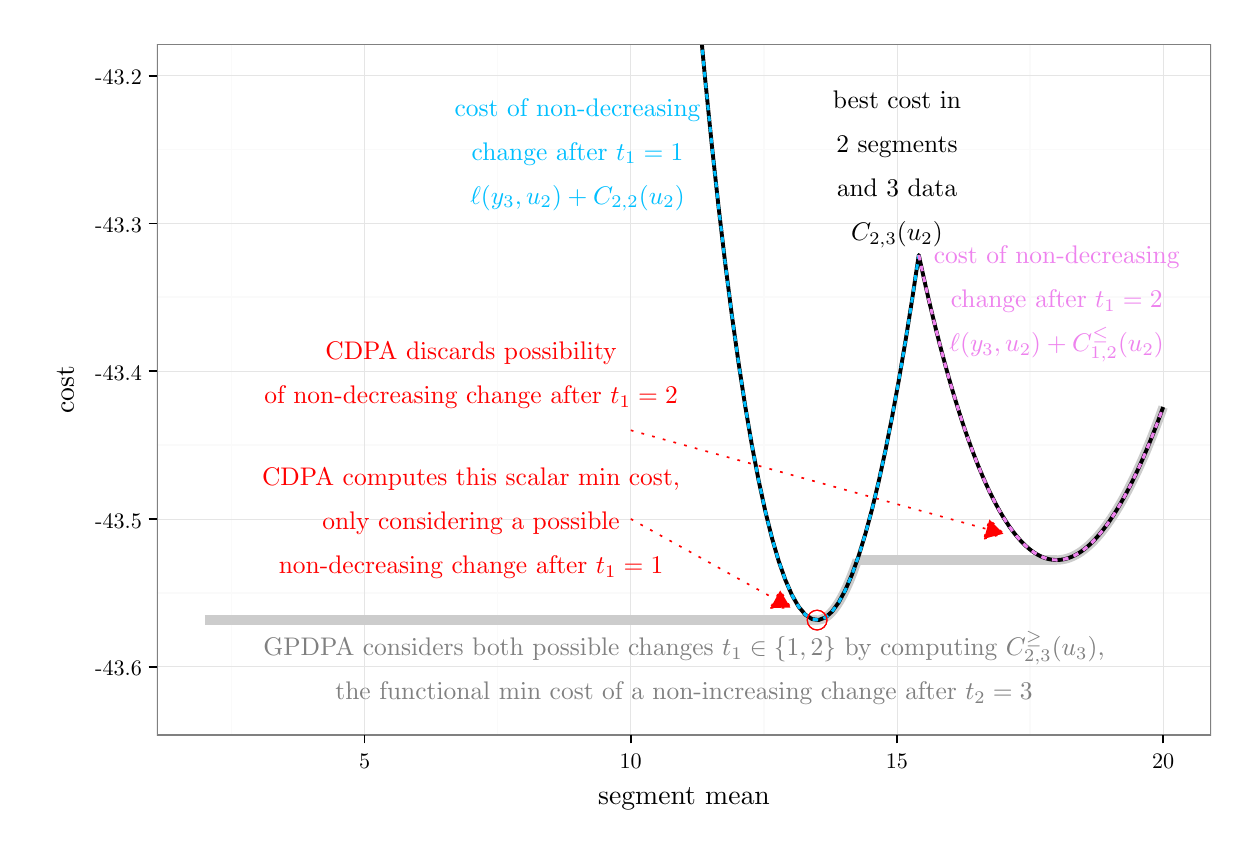
\begin{tikzpicture}[x=1pt,y=1pt]
\definecolor{fillColor}{RGB}{255,255,255}
\path[use as bounding box,fill=fillColor,fill opacity=0.00] (0,0) rectangle (433.62,289.08);
\begin{scope}
\path[clip] (  0.00,  0.00) rectangle (433.62,289.08);
\definecolor{drawColor}{RGB}{255,255,255}
\definecolor{fillColor}{RGB}{255,255,255}

\path[draw=drawColor,line width= 0.6pt,line join=round,line cap=round,fill=fillColor] (  0.00,  0.00) rectangle (433.62,289.08);
\end{scope}
\begin{scope}
\path[clip] ( 46.70, 33.48) rectangle (427.62,283.08);
\definecolor{fillColor}{RGB}{255,255,255}

\path[fill=fillColor] ( 46.70, 33.48) rectangle (427.62,283.08);
\definecolor{drawColor}{gray}{0.98}

\path[draw=drawColor,line width= 0.6pt,line join=round] ( 46.70, 84.87) --
	(427.62, 84.87);

\path[draw=drawColor,line width= 0.6pt,line join=round] ( 46.70,138.26) --
	(427.62,138.26);

\path[draw=drawColor,line width= 0.6pt,line join=round] ( 46.70,191.65) --
	(427.62,191.65);

\path[draw=drawColor,line width= 0.6pt,line join=round] ( 46.70,245.04) --
	(427.62,245.04);

\path[draw=drawColor,line width= 0.6pt,line join=round] ( 73.64, 33.48) --
	( 73.64,283.08);

\path[draw=drawColor,line width= 0.6pt,line join=round] (169.83, 33.48) --
	(169.83,283.08);

\path[draw=drawColor,line width= 0.6pt,line join=round] (266.02, 33.48) --
	(266.02,283.08);

\path[draw=drawColor,line width= 0.6pt,line join=round] (362.21, 33.48) --
	(362.21,283.08);
\definecolor{drawColor}{gray}{0.90}

\path[draw=drawColor,line width= 0.2pt,line join=round] ( 46.70, 58.17) --
	(427.62, 58.17);

\path[draw=drawColor,line width= 0.2pt,line join=round] ( 46.70,111.56) --
	(427.62,111.56);

\path[draw=drawColor,line width= 0.2pt,line join=round] ( 46.70,164.95) --
	(427.62,164.95);

\path[draw=drawColor,line width= 0.2pt,line join=round] ( 46.70,218.34) --
	(427.62,218.34);

\path[draw=drawColor,line width= 0.2pt,line join=round] ( 46.70,271.73) --
	(427.62,271.73);

\path[draw=drawColor,line width= 0.2pt,line join=round] (121.73, 33.48) --
	(121.73,283.08);

\path[draw=drawColor,line width= 0.2pt,line join=round] (217.92, 33.48) --
	(217.92,283.08);

\path[draw=drawColor,line width= 0.2pt,line join=round] (314.11, 33.48) --
	(314.11,283.08);

\path[draw=drawColor,line width= 0.2pt,line join=round] (410.31, 33.48) --
	(410.31,283.08);
\definecolor{drawColor}{gray}{0.80}

\path[draw=drawColor,line width= 3.4pt,line join=round] ( 64.02, 75.01) --
	( 66.25, 75.01) --
	( 68.49, 75.01) --
	( 70.72, 75.01) --
	( 72.96, 75.01) --
	( 75.19, 75.01) --
	( 77.43, 75.01) --
	( 79.66, 75.01) --
	( 81.90, 75.01) --
	( 84.13, 75.01) --
	( 86.37, 75.01) --
	( 88.60, 75.01) --
	( 90.84, 75.01) --
	( 93.07, 75.01) --
	( 95.30, 75.01) --
	( 97.54, 75.01) --
	( 99.77, 75.01) --
	(102.01, 75.01) --
	(104.24, 75.01) --
	(106.48, 75.01) --
	(108.71, 75.01) --
	(110.95, 75.01) --
	(113.18, 75.01) --
	(115.42, 75.01) --
	(117.65, 75.01) --
	(119.89, 75.01) --
	(122.12, 75.01) --
	(124.36, 75.01) --
	(126.59, 75.01) --
	(128.83, 75.01) --
	(131.06, 75.01) --
	(133.30, 75.01) --
	(135.53, 75.01) --
	(137.76, 75.01) --
	(140.00, 75.01) --
	(142.23, 75.01) --
	(144.47, 75.01) --
	(146.70, 75.01) --
	(148.94, 75.01) --
	(151.17, 75.01) --
	(153.41, 75.01) --
	(155.64, 75.01) --
	(157.88, 75.01) --
	(160.11, 75.01) --
	(162.35, 75.01) --
	(164.58, 75.01) --
	(166.82, 75.01) --
	(169.05, 75.01) --
	(171.29, 75.01) --
	(173.52, 75.01) --
	(175.76, 75.01) --
	(177.99, 75.01) --
	(180.22, 75.01) --
	(182.46, 75.01) --
	(184.69, 75.01) --
	(186.93, 75.01) --
	(189.16, 75.01) --
	(191.40, 75.01) --
	(193.63, 75.01) --
	(195.87, 75.01) --
	(198.10, 75.01) --
	(200.34, 75.01) --
	(202.57, 75.01) --
	(204.81, 75.01) --
	(207.04, 75.01) --
	(209.28, 75.01) --
	(211.51, 75.01) --
	(213.75, 75.01) --
	(215.98, 75.01) --
	(218.22, 75.01) --
	(220.45, 75.01) --
	(222.68, 75.01) --
	(224.92, 75.01) --
	(227.15, 75.01) --
	(229.39, 75.01) --
	(231.62, 75.01) --
	(233.86, 75.01) --
	(236.09, 75.01) --
	(238.33, 75.01) --
	(240.56, 75.01) --
	(242.80, 75.01) --
	(245.03, 75.01) --
	(247.27, 75.01) --
	(249.50, 75.01) --
	(251.74, 75.01) --
	(253.97, 75.01) --
	(256.21, 75.01) --
	(258.44, 75.01) --
	(260.68, 75.01) --
	(262.91, 75.01) --
	(265.14, 75.01) --
	(267.38, 75.01) --
	(269.61, 75.01) --
	(271.85, 75.01) --
	(274.08, 75.01) --
	(276.32, 75.01) --
	(278.55, 75.01) --
	(280.79, 75.01) --
	(283.02, 75.01) --
	(285.26, 75.01);

\path[draw=drawColor,line width= 3.4pt,line join=round] (285.26, 75.01) --
	(285.40, 75.01) --
	(285.55, 75.02) --
	(285.70, 75.03) --
	(285.84, 75.05) --
	(285.99, 75.07) --
	(286.14, 75.09) --
	(286.28, 75.12) --
	(286.43, 75.16) --
	(286.58, 75.20) --
	(286.72, 75.24) --
	(286.87, 75.29) --
	(287.02, 75.34) --
	(287.16, 75.40) --
	(287.31, 75.46) --
	(287.46, 75.52) --
	(287.60, 75.59) --
	(287.75, 75.67) --
	(287.90, 75.75) --
	(288.04, 75.83) --
	(288.19, 75.92) --
	(288.34, 76.02) --
	(288.48, 76.11) --
	(288.63, 76.21) --
	(288.78, 76.32) --
	(288.92, 76.43) --
	(289.07, 76.55) --
	(289.22, 76.67) --
	(289.36, 76.79) --
	(289.51, 76.92) --
	(289.66, 77.05) --
	(289.80, 77.19) --
	(289.95, 77.33) --
	(290.10, 77.48) --
	(290.24, 77.63) --
	(290.39, 77.79) --
	(290.54, 77.95) --
	(290.68, 78.11) --
	(290.83, 78.28) --
	(290.98, 78.45) --
	(291.12, 78.63) --
	(291.27, 78.81) --
	(291.41, 79.00) --
	(291.56, 79.19) --
	(291.71, 79.38) --
	(291.85, 79.58) --
	(292.00, 79.79) --
	(292.15, 80.00) --
	(292.29, 80.21) --
	(292.44, 80.43) --
	(292.59, 80.65) --
	(292.73, 80.87) --
	(292.88, 81.10) --
	(293.03, 81.34) --
	(293.17, 81.57) --
	(293.32, 81.82) --
	(293.47, 82.06) --
	(293.61, 82.32) --
	(293.76, 82.57) --
	(293.91, 82.83) --
	(294.05, 83.10) --
	(294.20, 83.37) --
	(294.35, 83.64) --
	(294.49, 83.92) --
	(294.64, 84.20) --
	(294.79, 84.48) --
	(294.93, 84.77) --
	(295.08, 85.07) --
	(295.23, 85.37) --
	(295.37, 85.67) --
	(295.52, 85.98) --
	(295.67, 86.29) --
	(295.81, 86.60) --
	(295.96, 86.92) --
	(296.11, 87.25) --
	(296.25, 87.58) --
	(296.40, 87.91) --
	(296.55, 88.25) --
	(296.69, 88.59) --
	(296.84, 88.93) --
	(296.99, 89.28) --
	(297.13, 89.63) --
	(297.28, 89.99) --
	(297.43, 90.35) --
	(297.57, 90.72) --
	(297.72, 91.09) --
	(297.87, 91.47) --
	(298.01, 91.85) --
	(298.16, 92.23) --
	(298.31, 92.62) --
	(298.45, 93.01) --
	(298.60, 93.40) --
	(298.75, 93.80) --
	(298.89, 94.21) --
	(299.04, 94.61) --
	(299.19, 95.03) --
	(299.33, 95.44) --
	(299.48, 95.86) --
	(299.62, 96.29) --
	(299.77, 96.72);

\path[draw=drawColor,line width= 3.4pt,line join=round] (299.77, 96.72) --
	(300.50, 96.72) --
	(301.23, 96.72) --
	(301.96, 96.72) --
	(302.68, 96.72) --
	(303.41, 96.72) --
	(304.14, 96.72) --
	(304.87, 96.72) --
	(305.59, 96.72) --
	(306.32, 96.72) --
	(307.05, 96.72) --
	(307.78, 96.72) --
	(308.51, 96.72) --
	(309.23, 96.72) --
	(309.96, 96.72) --
	(310.69, 96.72) --
	(311.42, 96.72) --
	(312.15, 96.72) --
	(312.87, 96.72) --
	(313.60, 96.72) --
	(314.33, 96.72) --
	(315.06, 96.72) --
	(315.78, 96.72) --
	(316.51, 96.72) --
	(317.24, 96.72) --
	(317.97, 96.72) --
	(318.70, 96.72) --
	(319.42, 96.72) --
	(320.15, 96.72) --
	(320.88, 96.72) --
	(321.61, 96.72) --
	(322.34, 96.72) --
	(323.06, 96.72) --
	(323.79, 96.72) --
	(324.52, 96.72) --
	(325.25, 96.72) --
	(325.97, 96.72) --
	(326.70, 96.72) --
	(327.43, 96.72) --
	(328.16, 96.72) --
	(328.89, 96.72) --
	(329.61, 96.72) --
	(330.34, 96.72) --
	(331.07, 96.72) --
	(331.80, 96.72) --
	(332.53, 96.72) --
	(333.25, 96.72) --
	(333.98, 96.72) --
	(334.71, 96.72) --
	(335.44, 96.72) --
	(336.16, 96.72) --
	(336.89, 96.72) --
	(337.62, 96.72) --
	(338.35, 96.72) --
	(339.08, 96.72) --
	(339.80, 96.72) --
	(340.53, 96.72) --
	(341.26, 96.72) --
	(341.99, 96.72) --
	(342.72, 96.72) --
	(343.44, 96.72) --
	(344.17, 96.72) --
	(344.90, 96.72) --
	(345.63, 96.72) --
	(346.35, 96.72) --
	(347.08, 96.72) --
	(347.81, 96.72) --
	(348.54, 96.72) --
	(349.27, 96.72) --
	(349.99, 96.72) --
	(350.72, 96.72) --
	(351.45, 96.72) --
	(352.18, 96.72) --
	(352.91, 96.72) --
	(353.63, 96.72) --
	(354.36, 96.72) --
	(355.09, 96.72) --
	(355.82, 96.72) --
	(356.54, 96.72) --
	(357.27, 96.72) --
	(358.00, 96.72) --
	(358.73, 96.72) --
	(359.46, 96.72) --
	(360.18, 96.72) --
	(360.91, 96.72) --
	(361.64, 96.72) --
	(362.37, 96.72) --
	(363.10, 96.72) --
	(363.82, 96.72) --
	(364.55, 96.72) --
	(365.28, 96.72) --
	(366.01, 96.72) --
	(366.73, 96.72) --
	(367.46, 96.72) --
	(368.19, 96.72) --
	(368.92, 96.72) --
	(369.65, 96.72) --
	(370.37, 96.72) --
	(371.10, 96.72) --
	(371.83, 96.72);

\path[draw=drawColor,line width= 3.4pt,line join=round] (371.83, 96.72) --
	(372.22, 96.72) --
	(372.61, 96.74) --
	(373.00, 96.77) --
	(373.38, 96.81) --
	(373.77, 96.87) --
	(374.16, 96.93) --
	(374.55, 97.01) --
	(374.94, 97.10) --
	(375.33, 97.20) --
	(375.72, 97.32) --
	(376.10, 97.44) --
	(376.49, 97.58) --
	(376.88, 97.73) --
	(377.27, 97.89) --
	(377.66, 98.06) --
	(378.05, 98.25) --
	(378.44, 98.44) --
	(378.83, 98.65) --
	(379.21, 98.87) --
	(379.60, 99.10) --
	(379.99, 99.34) --
	(380.38, 99.60) --
	(380.77, 99.86) --
	(381.16,100.14) --
	(381.55,100.43) --
	(381.93,100.73) --
	(382.32,101.04) --
	(382.71,101.36) --
	(383.10,101.70) --
	(383.49,102.04) --
	(383.88,102.40) --
	(384.27,102.77) --
	(384.65,103.15) --
	(385.04,103.54) --
	(385.43,103.94) --
	(385.82,104.35) --
	(386.21,104.78) --
	(386.60,105.21) --
	(386.99,105.66) --
	(387.38,106.12) --
	(387.76,106.59) --
	(388.15,107.07) --
	(388.54,107.56) --
	(388.93,108.06) --
	(389.32,108.57) --
	(389.71,109.10) --
	(390.10,109.63) --
	(390.48,110.18) --
	(390.87,110.74) --
	(391.26,111.30) --
	(391.65,111.88) --
	(392.04,112.47) --
	(392.43,113.07) --
	(392.82,113.68) --
	(393.21,114.30) --
	(393.59,114.94) --
	(393.98,115.58) --
	(394.37,116.23) --
	(394.76,116.90) --
	(395.15,117.57) --
	(395.54,118.26) --
	(395.93,118.96) --
	(396.31,119.66) --
	(396.70,120.38) --
	(397.09,121.11) --
	(397.48,121.85) --
	(397.87,122.60) --
	(398.26,123.36) --
	(398.65,124.13) --
	(399.03,124.91) --
	(399.42,125.70) --
	(399.81,126.50) --
	(400.20,127.31) --
	(400.59,128.13) --
	(400.98,128.96) --
	(401.37,129.81) --
	(401.76,130.66) --
	(402.14,131.52) --
	(402.53,132.40) --
	(402.92,133.28) --
	(403.31,134.17) --
	(403.70,135.08) --
	(404.09,135.99) --
	(404.48,136.92) --
	(404.86,137.85) --
	(405.25,138.79) --
	(405.64,139.75) --
	(406.03,140.71) --
	(406.42,141.69) --
	(406.81,142.67) --
	(407.20,143.67) --
	(407.59,144.67) --
	(407.97,145.69) --
	(408.36,146.71) --
	(408.75,147.75) --
	(409.14,148.79) --
	(409.53,149.84) --
	(409.92,150.91) --
	(410.31,151.98);
\definecolor{drawColor}{RGB}{0,0,0}

\node[text=drawColor,anchor=base,inner sep=0pt, outer sep=0pt, scale=  0.92] at (314.11,259.74) {best cost in};

\node[text=drawColor,anchor=base,inner sep=0pt, outer sep=0pt, scale=  0.92] at (314.11,243.85) {2 segments};

\node[text=drawColor,anchor=base,inner sep=0pt, outer sep=0pt, scale=  0.92] at (314.11,227.95) {and 3 data};

\node[text=drawColor,anchor=base,inner sep=0pt, outer sep=0pt, scale=  0.92] at (314.11,212.05) {$C_{2,3}(u_2)$};
\definecolor{drawColor}{RGB}{255,0,0}

\node[text=drawColor,anchor=base,inner sep=0pt, outer sep=0pt, scale=  0.92] at (160.21,169.10) {CDPA discards possibility};

\node[text=drawColor,anchor=base,inner sep=0pt, outer sep=0pt, scale=  0.92] at (160.21,153.20) {of non-decreasing change after $t_1=2$};

\path[draw=drawColor,line width= 0.6pt,dash pattern=on 1pt off 3pt ,line join=round] (217.92,143.60) -- (352.59,106.22);
\definecolor{fillColor}{RGB}{255,0,0}

\path[draw=drawColor,line width= 0.6pt,dash pattern=on 1pt off 3pt ,line join=round,fill=fillColor] (345.59,104.41) --
	(352.59,106.22) --
	(347.53,111.38) --
	cycle;

\node[text=drawColor,anchor=base,inner sep=0pt, outer sep=0pt, scale=  0.92] at (160.21,123.66) {CDPA computes this scalar min cost,};

\node[text=drawColor,anchor=base,inner sep=0pt, outer sep=0pt, scale=  0.92] at (160.21,107.76) {only considering a possible};

\node[text=drawColor,anchor=base,inner sep=0pt, outer sep=0pt, scale=  0.92] at (160.21, 91.86) {non-decreasing change after $t_1=1$};

\path[draw=drawColor,line width= 0.6pt,dash pattern=on 1pt off 3pt ,line join=round] (217.92,111.56) -- (275.64, 79.53);

\path[draw=drawColor,line width= 0.6pt,dash pattern=on 1pt off 3pt ,line join=round,fill=fillColor] (268.41, 79.40) --
	(275.64, 79.53) --
	(271.92, 85.72) --
	cycle;
\definecolor{drawColor}{gray}{0.50}

\node[text=drawColor,anchor=base,inner sep=0pt, outer sep=0pt, scale=  0.92] at (237.16, 62.32) {GPDPA considers both possible changes $t_1\in\{1,2\}$ by computing $C^\geq_{2,3}(u_3)$,};

\node[text=drawColor,anchor=base,inner sep=0pt, outer sep=0pt, scale=  0.92] at (237.16, 46.42) {the functional min cost of a non-increasing change after $t_2=3$};
\definecolor{drawColor}{RGB}{0,0,0}

\path[draw=drawColor,line width= 1.4pt,line join=round] (243.05,289.08) --
	(244.83,270.22) --
	(247.24,246.41) --
	(249.65,224.30) --
	(252.06,203.86) --
	(254.47,185.06) --
	(256.89,167.85) --
	(259.30,152.22) --
	(261.71,138.11) --
	(264.12,125.51) --
	(266.53,114.39) --
	(268.94,104.70) --
	(271.35, 96.43) --
	(273.77, 89.55) --
	(276.18, 84.03) --
	(278.59, 79.84) --
	(281.00, 76.97) --
	(283.41, 75.38) --
	(285.82, 75.04) --
	(288.24, 75.95) --
	(290.65, 78.07) --
	(293.06, 81.39) --
	(295.47, 85.87) --
	(297.88, 91.51) --
	(300.29, 98.27) --
	(302.70,106.15) --
	(305.12,115.12) --
	(307.53,125.16) --
	(309.94,136.25) --
	(312.35,148.39) --
	(314.76,161.54) --
	(317.17,175.69) --
	(319.59,190.83) --
	(322.00,206.94) --
	(322.00,206.94) --
	(322.89,202.82) --
	(323.78,198.79) --
	(324.67,194.84) --
	(325.56,190.98) --
	(326.46,187.21) --
	(327.35,183.52) --
	(328.24,179.91) --
	(329.13,176.39) --
	(330.02,172.95) --
	(330.92,169.59) --
	(331.81,166.31) --
	(332.70,163.12) --
	(333.59,160.01) --
	(334.48,156.97) --
	(335.38,154.02) --
	(336.27,151.15) --
	(337.16,148.36) --
	(338.05,145.64) --
	(338.94,143.00) --
	(339.84,140.44) --
	(340.73,137.96) --
	(341.62,135.56) --
	(342.51,133.23) --
	(343.40,130.98) --
	(344.30,128.80) --
	(345.19,126.70) --
	(346.08,124.68) --
	(346.97,122.73) --
	(347.86,120.85) --
	(348.76,119.04) --
	(349.65,117.31) --
	(350.54,115.66) --
	(351.43,114.07) --
	(352.32,112.56) --
	(353.22,111.12) --
	(354.11,109.74) --
	(355.00,108.45) --
	(355.89,107.22) --
	(356.79,106.06) --
	(357.68,104.97) --
	(358.57,103.95) --
	(359.46,103.00) --
	(360.35,102.11) --
	(361.25,101.30) --
	(362.14,100.55) --
	(363.03, 99.87) --
	(363.92, 99.26) --
	(364.81, 98.72) --
	(365.71, 98.24) --
	(366.60, 97.82) --
	(367.49, 97.48) --
	(368.38, 97.20) --
	(369.27, 96.98) --
	(370.17, 96.83) --
	(371.06, 96.74) --
	(371.95, 96.72) --
	(372.84, 96.76) --
	(373.73, 96.86) --
	(374.63, 97.03) --
	(375.52, 97.26) --
	(376.41, 97.55) --
	(377.30, 97.90) --
	(378.19, 98.32) --
	(379.09, 98.80) --
	(379.98, 99.33) --
	(380.87, 99.93) --
	(381.76,100.59) --
	(382.65,101.31) --
	(383.55,102.09) --
	(384.44,102.93) --
	(385.33,103.83) --
	(386.22,104.79) --
	(387.11,105.81) --
	(388.01,106.89) --
	(388.90,108.02) --
	(389.79,109.21) --
	(390.68,110.46) --
	(391.57,111.77) --
	(392.47,113.13) --
	(393.36,114.55) --
	(394.25,116.03) --
	(395.14,117.56) --
	(396.03,119.15) --
	(396.93,120.80) --
	(397.82,122.50) --
	(398.71,124.25) --
	(399.60,126.06) --
	(400.49,127.93) --
	(401.39,129.85) --
	(402.28,131.82) --
	(403.17,133.85) --
	(404.06,135.93) --
	(404.95,138.07) --
	(405.85,140.25) --
	(406.74,142.49) --
	(407.63,144.79) --
	(408.52,147.13) --
	(409.41,149.53) --
	(410.31,151.98);
\definecolor{drawColor}{RGB}{0,191,255}

\path[draw=drawColor,line width= 1.1pt,dash pattern=on 2pt off 2pt ,line join=round] (243.05,289.08) --
	(244.83,270.22) --
	(247.24,246.41) --
	(249.65,224.30) --
	(252.06,203.86) --
	(254.47,185.06) --
	(256.89,167.85) --
	(259.30,152.22) --
	(261.71,138.11) --
	(264.12,125.51) --
	(266.53,114.39) --
	(268.94,104.70) --
	(271.35, 96.43) --
	(273.77, 89.55) --
	(276.18, 84.03) --
	(278.59, 79.84) --
	(281.00, 76.97) --
	(283.41, 75.38) --
	(285.82, 75.04) --
	(288.24, 75.95) --
	(290.65, 78.07) --
	(293.06, 81.39) --
	(295.47, 85.87) --
	(297.88, 91.51) --
	(300.29, 98.27) --
	(302.70,106.15) --
	(305.12,115.12) --
	(307.53,125.16) --
	(309.94,136.25) --
	(312.35,148.39) --
	(314.76,161.54) --
	(317.17,175.69) --
	(319.59,190.83) --
	(322.00,206.94);
\definecolor{drawColor}{RGB}{238,130,238}

\path[draw=drawColor,line width= 1.1pt,dash pattern=on 2pt off 2pt ,line join=round] (322.00,206.94) --
	(322.89,202.82) --
	(323.78,198.79) --
	(324.67,194.84) --
	(325.56,190.98) --
	(326.46,187.21) --
	(327.35,183.52) --
	(328.24,179.91) --
	(329.13,176.39) --
	(330.02,172.95) --
	(330.92,169.59) --
	(331.81,166.31) --
	(332.70,163.12) --
	(333.59,160.01) --
	(334.48,156.97) --
	(335.38,154.02) --
	(336.27,151.15) --
	(337.16,148.36) --
	(338.05,145.64) --
	(338.94,143.00) --
	(339.84,140.44) --
	(340.73,137.96) --
	(341.62,135.56) --
	(342.51,133.23) --
	(343.40,130.98) --
	(344.30,128.80) --
	(345.19,126.70) --
	(346.08,124.68) --
	(346.97,122.73) --
	(347.86,120.85) --
	(348.76,119.04) --
	(349.65,117.31) --
	(350.54,115.66) --
	(351.43,114.07) --
	(352.32,112.56) --
	(353.22,111.12) --
	(354.11,109.74) --
	(355.00,108.45) --
	(355.89,107.22) --
	(356.79,106.06) --
	(357.68,104.97) --
	(358.57,103.95) --
	(359.46,103.00) --
	(360.35,102.11) --
	(361.25,101.30) --
	(362.14,100.55) --
	(363.03, 99.87) --
	(363.92, 99.26) --
	(364.81, 98.72) --
	(365.71, 98.24) --
	(366.60, 97.82) --
	(367.49, 97.48) --
	(368.38, 97.20) --
	(369.27, 96.98) --
	(370.17, 96.83) --
	(371.06, 96.74) --
	(371.95, 96.72) --
	(372.84, 96.76) --
	(373.73, 96.86) --
	(374.63, 97.03) --
	(375.52, 97.26) --
	(376.41, 97.55) --
	(377.30, 97.90) --
	(378.19, 98.32) --
	(379.09, 98.80) --
	(379.98, 99.33) --
	(380.87, 99.93) --
	(381.76,100.59) --
	(382.65,101.31) --
	(383.55,102.09) --
	(384.44,102.93) --
	(385.33,103.83) --
	(386.22,104.79) --
	(387.11,105.81) --
	(388.01,106.89) --
	(388.90,108.02) --
	(389.79,109.21) --
	(390.68,110.46) --
	(391.57,111.77) --
	(392.47,113.13) --
	(393.36,114.55) --
	(394.25,116.03) --
	(395.14,117.56) --
	(396.03,119.15) --
	(396.93,120.80) --
	(397.82,122.50) --
	(398.71,124.25) --
	(399.60,126.06) --
	(400.49,127.93) --
	(401.39,129.85) --
	(402.28,131.82) --
	(403.17,133.85) --
	(404.06,135.93) --
	(404.95,138.07) --
	(405.85,140.25) --
	(406.74,142.49) --
	(407.63,144.79) --
	(408.52,147.13) --
	(409.41,149.53) --
	(410.31,151.98);
\definecolor{drawColor}{RGB}{255,0,0}

\path[draw=drawColor,line width= 0.4pt,line join=round,line cap=round] (285.26, 75.01) circle (  3.57);

\path[draw=drawColor,line width= 0.4pt,line join=round,line cap=round] (285.26, 75.01) circle (  3.57);
\definecolor{drawColor}{RGB}{0,191,255}

\node[text=drawColor,anchor=base,inner sep=0pt, outer sep=0pt, scale=  0.92] at (198.69,257.13) {cost of non-decreasing};

\node[text=drawColor,anchor=base,inner sep=0pt, outer sep=0pt, scale=  0.92] at (198.69,241.24) {change after $t_1=1$};

\node[text=drawColor,anchor=base,inner sep=0pt, outer sep=0pt, scale=  0.92] at (198.69,225.34) {$\ell(y_3, u_2)+C_{2,2}(u_2)$};
\definecolor{drawColor}{RGB}{238,130,238}

\node[text=drawColor,anchor=base,inner sep=0pt, outer sep=0pt, scale=  0.92] at (371.83,203.74) {cost of non-decreasing};

\node[text=drawColor,anchor=base,inner sep=0pt, outer sep=0pt, scale=  0.92] at (371.83,187.85) {change after $t_1=2$};

\node[text=drawColor,anchor=base,inner sep=0pt, outer sep=0pt, scale=  0.92] at (371.83,171.95) {$\ell(y_3, u_2)+C^\leq_{1,2}(u_2)$};
\definecolor{drawColor}{gray}{0.50}

\path[draw=drawColor,line width= 0.6pt,line join=round,line cap=round] ( 46.70, 33.48) rectangle (427.62,283.08);
\end{scope}
\begin{scope}
\path[clip] (  0.00,  0.00) rectangle (433.62,289.08);
\definecolor{drawColor}{RGB}{0,0,0}

\node[text=drawColor,anchor=base east,inner sep=0pt, outer sep=0pt, scale=  0.80] at ( 41.30, 54.86) {-43.6};

\node[text=drawColor,anchor=base east,inner sep=0pt, outer sep=0pt, scale=  0.80] at ( 41.30,108.26) {-43.5};

\node[text=drawColor,anchor=base east,inner sep=0pt, outer sep=0pt, scale=  0.80] at ( 41.30,161.65) {-43.4};

\node[text=drawColor,anchor=base east,inner sep=0pt, outer sep=0pt, scale=  0.80] at ( 41.30,215.04) {-43.3};

\node[text=drawColor,anchor=base east,inner sep=0pt, outer sep=0pt, scale=  0.80] at ( 41.30,268.43) {-43.2};
\end{scope}
\begin{scope}
\path[clip] (  0.00,  0.00) rectangle (433.62,289.08);
\definecolor{drawColor}{RGB}{0,0,0}

\path[draw=drawColor,line width= 0.6pt,line join=round] ( 43.70, 58.17) --
	( 46.70, 58.17);

\path[draw=drawColor,line width= 0.6pt,line join=round] ( 43.70,111.56) --
	( 46.70,111.56);

\path[draw=drawColor,line width= 0.6pt,line join=round] ( 43.70,164.95) --
	( 46.70,164.95);

\path[draw=drawColor,line width= 0.6pt,line join=round] ( 43.70,218.34) --
	( 46.70,218.34);

\path[draw=drawColor,line width= 0.6pt,line join=round] ( 43.70,271.73) --
	( 46.70,271.73);
\end{scope}
\begin{scope}
\path[clip] (  0.00,  0.00) rectangle (433.62,289.08);
\definecolor{drawColor}{RGB}{0,0,0}

\path[draw=drawColor,line width= 0.6pt,line join=round] (121.73, 30.48) --
	(121.73, 33.48);

\path[draw=drawColor,line width= 0.6pt,line join=round] (217.92, 30.48) --
	(217.92, 33.48);

\path[draw=drawColor,line width= 0.6pt,line join=round] (314.11, 30.48) --
	(314.11, 33.48);

\path[draw=drawColor,line width= 0.6pt,line join=round] (410.31, 30.48) --
	(410.31, 33.48);
\end{scope}
\begin{scope}
\path[clip] (  0.00,  0.00) rectangle (433.62,289.08);
\definecolor{drawColor}{RGB}{0,0,0}

\node[text=drawColor,anchor=base,inner sep=0pt, outer sep=0pt, scale=  0.80] at (121.73, 21.46) {5};

\node[text=drawColor,anchor=base,inner sep=0pt, outer sep=0pt, scale=  0.80] at (217.92, 21.46) {10};

\node[text=drawColor,anchor=base,inner sep=0pt, outer sep=0pt, scale=  0.80] at (314.11, 21.46) {15};

\node[text=drawColor,anchor=base,inner sep=0pt, outer sep=0pt, scale=  0.80] at (410.31, 21.46) {20};
\end{scope}
\begin{scope}
\path[clip] (  0.00,  0.00) rectangle (433.62,289.08);
\definecolor{drawColor}{RGB}{0,0,0}

\node[text=drawColor,anchor=base,inner sep=0pt, outer sep=0pt, scale=  1.00] at (237.16,  8.40) {segment mean};
\end{scope}
\begin{scope}
\path[clip] (  0.00,  0.00) rectangle (433.62,289.08);
\definecolor{drawColor}{RGB}{0,0,0}

\node[text=drawColor,rotate= 90.00,anchor=base,inner sep=0pt, outer sep=0pt, scale=  1.00] at ( 16.66,158.28) {cost};
\end{scope}
\end{tikzpicture}



\section{Algorithm pseudocode}

\subsection{GPDPA for reduced isotonic regression}
In this section we give pseudocode for our proposed Generalized Pruned
Dynamic Programming Algorithm (GPDPA) for the reduced isotonic
regression problem. We propose the following data structures and
sub-routines for the computation:
\begin{itemize}
\item FunctionPiece: a data structure which represents one piece of a
  $C_{k,t}(u)$ cost function (for one interval of mean values $u$). It
  has coefficients which depend on the convex loss function $\ell$
  (for the square loss it has three real-valued coefficients $a,b,c$
  which define a function $au^2 + bu + c$). It also has two
  real-valued elements for min/max mean values
  $[\underline u, \overline u]$ of this interval, meaning the function
  $C_{k,t}(u)=au^2 + bu + c$ for all
  $u\in[\underline u, \overline u]$. Finally it stores a previous
  segment endpoint $t'$ (integer) and mean $u'$ (real).
\item FunctionPieceList: an ordered list of FunctionPiece objects,
  which exactly stores a cost function $\FCC_{k,t}(u)$ for all values
  of last segment mean $u$.
\item $\text{OnePiece}(y, \underline u, \overline u)$: a sub-routine
  that initializes a FunctionPieceList with just one FunctionPiece
  $\ell(y, u)$ defined on $[\underline u, \overline u]$.
\item $\text{MinLess}(t, f)$: an algorithm that inputs a changepoint
  and a FunctionPieceList, and outputs the corresponding min-less
  operator $f^\leq$ (another FunctionPieceList), with the previous
  changepoint set to $t'=t$ for each of its pieces. This algorithm
  also needs to store the previous mean value $u'$ for each of the
  function pieces (see pseudocode below). 
\item $\text{MinOfTwo} (f_1, f_2)$: an algorithm that inputs two
  FunctionPieceList objects, and outputs another FunctionPieceList
  object which is their minimum. 
\item $\text{ArgMin}(f)$: an algorithm that inputs a FunctionPieceList
  and outputs three values: the optimal mean $u^*=\argmin_u f(u)$, the
  previous segment end $t'$ and mean $u'$.
\item $\text{FindMean}(u, f)$ an algorithm that inputs a mean value
  and a FunctionPieceList. It finds the FunctionPiece in $f$ with mean
  $u\in[\underline u, \overline u]$ contained in its interval, then
  outputs the previous segment end $t'$ and mean $u'$ stored in that
  FunctionPiece.
\end{itemize}
The above data structures and sub-routines are used in the following
pseudo-code, which describes the GPDPA for solving the reduced
isotonic regression problem.
\begin{algorithm}[H]
\begin{algorithmic}[1]
\STATE Input: data set $\mathbf y\in\RR^n$, maximum number of segments $K\in\{2,\dots, n\}$.
\STATE Output: matrices of optimal segment means $U\in\RR^{K\times K}$ 
and ends $T\in\{1,\dots,n\}^{K\times K}$
\STATE Compute min $\underline y$ and max $\overline y$ of $\mathbf y$.
\label{line:min-max}
\STATE $\FCC_{1,1}\gets \text{OnePiece}(y_1, \underline y, \overline y)$
\label{line:init-1}
\STATE for data points $t$ from 2 to $n$:
\begin{ALC@g}
  \STATE $\FCC_{1,t}\gets \text{OnePiece}(y_t, \underline y, \overline y) + \FCC_{1,t-1}$
\label{line:init-t}
\end{ALC@g}
\STATE for segments $k$ from 2 to $K$: for data points $t$ from $k$ to $n$: // dynamic programming
\label{line:for-k-t}
\begin{ALC@g}
  \STATE $\text{min\_prev}\gets \text{MinLess}(t-1, \FCC_{k-1,t-1})$ // this is $\FCC_{k-1,t-1}^\leq$
  \label{line:MinLess}
  % \STATE if $t=k$:
  % \begin{ALC@g}
  %   \STATE $\text{min\_new}\gets\text{min\_prev}$ // there is only one
  %   possible changepoint, before $t$
  % \end{ALC@g}
  % \STATE else:
  % \begin{ALC@g}
  %   \STATE $\text{min\_new}\gets\text{MinOfTwo}(\text{min\_prev}, \FCC_{k, t-1})$
  % \end{ALC@g}
    \STATE $\text{min\_new}\gets\text{min\_prev}$ if $t=k$, 
else $\text{MinOfTwo}(\text{min\_prev}, \FCC_{k, t-1})$
  \label{line:MinOfTwo}
  \STATE $\FCC_{k,t}\gets \text{min\_new} + \text{OnePiece}(y_t, \underline y, \overline y)$
  \label{line:AddNew}
\end{ALC@g}
\STATE for segments $k$ from 1 to $K$: // decoding for every model size $k$
\label{line:for-k-decoding}
\begin{ALC@g}
  \STATE $u^*,t',u'\gets \text{ArgMin}(\FCC_{k,n})$
  \label{line:ArgMin}
  \STATE $U_{k,k}\gets u^*;\, T_{k,k}\gets t'$ // store mean of segment $k$ and end of segment $k-1$
  \label{line:decode-kk}
  \STATE for segment $s$ from $k-1$ to $1$: // decoding for every segment $s<k$
  \label{line:for-s-decoding}
  \begin{ALC@g}
    \STATE if $u' < \infty$: $u^*\gets u'$ // equality constraint active, $u_s = u_{s+1}$
    \label{line:equality-constraint-active}
    \STATE $t',u'\gets\text{FindMean}(u^*, \FCC_{s,t'})$
    \label{line:FindMean}
    \STATE $U_{k,s}\gets u^*;\, T_{k,s}\gets t'$ // store mean of segment $s$ and end of segment $s-1$
    \label{line:decode-ks}
  \end{ALC@g}
\end{ALC@g}
\caption{\label{algo:SNIR}Generalized Pruned Dynamic Programming
  Algorithm (GPDPA) for solving the reduced isotonic regression
  problem.}
\end{algorithmic}
\end{algorithm}

Algorithm~\ref{algo:SNIR} begins by computing the min/max on
line~\ref{line:min-max}.  The main storage of the algorithm is
$\FCC_{k,t}$, which should be initialized as a $K\times n$ array of
empty FunctionPieceList objects. The computation of $\FCC_{1,t}$ for
all $t$ occurs on lines~\ref{line:init-1}--\ref{line:init-t}. 

The dynamic programming updates occur in the for loops on
lines~\ref{line:for-k-t}--\ref{line:AddNew}. Line~\ref{line:MinLess}
uses the MinLess sub-routine to compute the temporary
FunctionPieceList min\_prev (which represents the function
$\FCC_{k-1,t-1}^\leq$). Line~\ref{line:MinOfTwo} sets the temporary
FunctionPieceList min\_new to the cost of the only possible
changepoint if $t=k$; otherwise, it uses the MinOfTwo sub-routine to
compute the cost of the best changepoint for every possible mean
value. Line~\ref{line:AddNew} adds the cost of data point $t$, and
stores the resulting FunctionPieceList in $\FCC_{k,t}$.

The decoding of the optimal segment mean $U$ (a $K\times K$ array of
real numbers) and end $T$ (a $K\times K$ array of integers) variables
occurs in the for loops on
lines~\ref{line:for-k-decoding}--\ref{line:decode-ks}. For a given
model size $k$, the decoding begins on line~\ref{line:ArgMin} by using
the ArgMin sub-routine to solve $u^* = \argmin_u \FCC_{k,n}(u)$ (the
optimal values for the previous segment end $t'$ and mean $u'$ are
also returned). Now we know that $u^*$ is the optimal mean of the last
($k$-th) segment, which occurs from data point $t'+1$ to $n$. These
values are stored in $U_{k,k}$ and $T_{k,k}$
(line~\ref{line:decode-kk}). And we already know that the optimal mean
of segment $k-1$ is $u'$.  Note that the $u'=\infty$ flag means that
the equality constraint is active
(line~\ref{line:equality-constraint-active}). The decoding of the
other segments $s<k$ proceeds using the FindMean sub-routine
(line~\ref{line:FindMean}). It takes the cost $\FCC_{s,t'}$ of the
best model in $s$ segments up to data point $t'$, finds the
FunctionPiece that stores the cost of $u^*$, and returns the new
optimal values of the previous segment end $t'$ and mean $u'$. The
mean of segment $s$ is stored in $U_{k,s}$ and the end of segment
$s-1$ is stored in $T_{k,s}$ (line~\ref{line:decode-ks}).

The time complexity of Algorithm~\ref{algo:SNIR} is $O(K n I)$ where
$I$ is the complexity of the MinLess and MinOfTwo sub-routines, which
is linear in the number of intervals (FunctionPiece objects) that are
used to represent the cost functions. There are pathological synthetic
data sets for which the number of intervals $I=O(n)$, implying a
time complexity of $O(K n^2)$. However, the average number
of intervals in real data sets is empirically $I=O(\log n)$, so the
average time complexity of Algorithm~\ref{algo:SNIR} is
$O(K n \log n)$.

\subsection{Min-less algorithm}

The following sub-routines are used to implement the MinLess algorithm.

\begin{itemize}
\item $\text{GetCost}(p, u)$: an algorithm that takes a FunctionPiece
  object $p$, and a mean value $u$, and computes the cost at $u$. For
  a square loss FunctionPiece $p$ with coefficients $a,b,c\in\RR$, we
  have $\text{GetCost}(p,u)=au^2+bu+c$.
\item $\text{OptimalMean}(p)$: an algorithm that takes one
  FunctionPiece object, and computes the optimal mean value. For a
  square loss FunctionPiece $p$ we have
  $\text{OptimalMean}(p)=-b/(2a)$.
\item $\text{ComputeRoots}(p, d)$: an algorithm that takes one
  FunctionPiece object, and computes the solutions to $p(u)=d$. For
  the square loss we propose to use the quadratic formula. For other
  convex losses that do not have closed form expressions for their
  roots, we propose to use Newton's root finding method. Note that for
  some constants $d$ there are no roots, and the algorithm needs to
  report that.
\item $f.\text{push\_piece}(\underline u, \overline u, p, u')$: push a
  new FunctionPiece at the end of FunctionPieceList $f$, with
  coefficients defined by FunctionPiece $p$, on interval
  $[\underline u, \overline u]$, with previous segment mean set to
  $u'$.
\item $\text{ConstPiece}(c)$: sub-routine that initializes a
  FunctionPiece $p$ with constant cost $c$ (for the square loss it
  sets $a=b=0$ in $au^2 + bu + c$).
\end{itemize}

\begin{algorithm}[H]
\begin{algorithmic}[1]
\STATE Input: The previous segment end $t_{\text{prev}}$ (an integer), 
 and $f_{\text{in}}$ (a FunctionPieceList).
\STATE Output: FunctionPieceList $f_{\text{out}}$, initialized as an empty list.
\STATE $\text{prev\_cost} \gets\infty$
\STATE $\text{new\_lower\_limit}\gets \text{LowerLimit}(f_{\text{in}}[0])$.
\STATE $i\gets 0$; // start at FunctionPiece on the left
\STATE while $i < $ Length($f_{\text{in}}$): // continue until FunctionPiece on the right
\begin{ALC@g}
  \STATE FunctionPiece $p\gets f_{\text{in}}[i]$
  \STATE if prev\_cost = $\infty$: // look for min in this interval.
  \begin{ALC@g}
    \STATE $\text{candidate\_mean}\gets \text{OptimalMean}(p)$ 
    \STATE if $\text{LowerLimit}(p)< \text{candidate\_mean} < \text{UpperLimit}(p)$:
    \begin{ALC@g}
      \STATE $\text{new\_upper\_limit}\gets \text{candidate\_mean}$ // Minimum found in this interval.
      \STATE $\text{prev\_cost}\gets \text{GetCost}(p, \text{candidate\_mean})$
      \STATE $\text{prev\_mean}\gets \text{candidate\_mean}$
    \end{ALC@g}
    \STATE else: // No minimum in this interval.
    \begin{ALC@g}
      \STATE 
      $\text{new\_upper\_limit}\gets
 \text{UpperLimit}(p)$
    \end{ALC@g}
    \STATE $f_{\text{out}}\text{.push\_piece}(\text{new\_lower\_limit},\text{new\_upper\_limit},p,\infty)$
    \STATE $\text{new\_lower\_limit}\gets\text{new\_upper\_limit}$
    \STATE $i\gets i+1$
  \end{ALC@g}
  \STATE else: // look for equality of $p$ and prev\_cost
  \begin{ALC@g}
    \STATE $(\text{small\_root},\text{large\_root})\gets\text{ComputeRoots}(p, \text{prev\_cost})$
    \STATE if $\text{LowerLimit}(p) < \text{small\_root} < \text{UpperLimit}(p)$:
    \begin{ALC@g}
      \STATE $f_{\text{out}}\text{.push\_piece}(
      \text{new\_lower\_limit}, 
      \text{small\_root}, 
      \text{ConstPiece}(\text{prev\_cost}), 
      \text{prev\_mean})$
      \STATE $\text{new\_lower\_limit}\gets \text{small\_root}$
      \STATE $\text{prev\_cost}\gets \infty$ 
    \end{ALC@g}
    \STATE else: // no equality in this interval
    \begin{ALC@g}
      \STATE $i\gets i+1$ // continue to next FunctionPiece
    \end{ALC@g}
  \end{ALC@g}
\end{ALC@g}
  \STATE if $\text{prev\_cost} < \infty$: // ending on constant piece
  \begin{ALC@g}
    \STATE $f_{\text{out}}\text{.push\_piece}(
    \text{new\_lower\_limit}, 
    \text{UpperLimit}(p), 
    \text{ConstPiece}(\text{prev\_cost}), 
    \text{prev\_mean})$
  \end{ALC@g}
\STATE Set all previous segment end $t'=t_{\text{prev}}$  for all FunctionPieces in $f_{\text{out}}$
\caption{\label{algo:minless}MinLess algorithm.}
\end{algorithmic}
\end{algorithm}

Consider Algorithm~\ref{algo:minless} which contains pseudocode for
the computation of the min-less operator. The algorithm initializes
prev\_cost (line~3), which is a state variable that is used on line~8
to decide whether the algorithm should look for a local minimum or an
intersection with a finite cost. Since prev\_cost is initially set to
$\infty$, the algorithm begins by following the convex function pieces
from left to right until finding a local minimum. If no minimum is found in
a given convex FunctionPiece (line~15), it is simply pushed on to the
end of the new FunctionPieceList (line~16). If a minimum occurs within
an interval (line~10), the cost and mean are stored (lines 11--12),
and a new convex FunctionPiece is created with upper limit ending at
that mean value (line~16). Then the algorithm starts looking for
another FunctionPiece with the same cost, by computing the smaller
root of the convex loss function (line~20). When a FunctionPiece is
found with a root in the interval (line~21), a new constant
FunctionPiece is pushed (line~22), and the algorithm resumes searching
for a minimum. At the end of the algorithm, a constant FunctionPiece
is pushed if necessary (line~28). The complexity of this algorithm is
$O(I)$ where $I$ is the number of FunctionPiece objects in
$f_\text{in}$.

The algorithm which implements the min-more operator is
analogous. Rather than searching from left to right, it searches from
right to left. Rather than using the small root (line~21), it uses the
large root.

\subsection{Implementation details}

Some implementation details that we found to be important:
\begin{description}
\item[Weights] for data sequences that contain repeats it is
  computationally advantageous to use a run-length encoding of the
  data, and a corresponding loss function. For example if the data
  sequence 5,1,1,1,0,0,5,5 is encoded as $n=4$ counts $y_t$ 5,1,0,5 with
  corresponding weights $w_t$ 1,3,2,2 then the Poisson loss function
  for mean $\mu$ is $\ell(y_t, w_t, \mu) = w_t(\mu- y_t\log \mu)$.
\item[Mean cost] The text defines $C_{k,t}$ functions as the total
  cost. However for very large data sets the cost values will be very
  large, resulting in numerical instability. To overcome this issue we
  instead implemented update rules using the mean cost.  For weights
  $W_{t}=\sum_{i=1}^t w_i$, the update rule to compute the mean cost is
$$  C_{k,t}(\mu) = \frac{1}{W_{t}} \left[\ell(y_t, \mu) + 
W_{t-1}
\min\{ C_{k,t-1}(\mu),\, C_{k-1,t-1}^\leq(\mu)  \}\right]$$
\item[Intervals in log(mean) space] For the Poisson model of
  non-negative count data $y_t\in\{0,1,2,\dots\}$ there is no possible
  mean $\mu$ value less than 0. We thus used $\log(\mu)$ values to
  implement intervals in FunctionPiece objects. For example rather
  than storing $\mu\in[0,1]$ we store $\log\mu\in[-\infty, 0]$.
\item[Root finding] For the ComputeRoots sub-routine for the Poisson
  loss, we used Newton root finding. For the larger root we solve
  $a\log\mu + b\mu + c = 0$ (linear as $\mu\rightarrow\infty$) and for
  the smaller root we solve $a x + be^x + c = 0$ ($x=\log \mu$, linear
  as $x\rightarrow -\infty$ and $\mu\rightarrow 0$). We stop the root
  finding when the cost is near zero (absolute cost value less
  than $10^{-12}$).
\item[Storage] Since the dynamic programming update rule for $C_{k,t}$
  only depends on $C_{k-1,t-1}^\geq$ and $C_{k,t-1}$, these are the
  only functions that need to be in memory, and the rest of the cost
  functions can be stored on disk (until the decoding step). We used
  the Berkeley DB Standard Template Library to store all the $C_{k,t}$
  as a vector of FunctionPieceList objects.
\end{description}

\end{document}